% !TeX root = Notizen.tex

\section*{Aufgabe 1: Doppelpendel}
\subsection*{a)}
Die Orte der Massen $m_1$ und $m_2$ im Doppelpendel sind:
\begin{align}
\vec{r_1}=\begin{pmatrix}\sin(\theta_1)\\-\cos(\theta_1)\end{pmatrix}
\cdot\SI{1}{m}~~\text{und}~~
\vec{r_2}=\begin{pmatrix}\sin(\theta_1)+\sin(\theta_2)\\-\cos(\theta_1)-\cos(\theta_2)\end{pmatrix}\cdot\SI{1}{m}.
\end{align}
Die Geschwindigkeiten sind also:
\begin{align}
\dot{\vec{r_1}}=\begin{pmatrix}\dot{\theta_1}\cos(\theta_1)\\\dot\theta_1\sin(\theta_1)\end{pmatrix}\cdot\SI{1}{\meter\per\second}
~~\text{und}~~
\vec{r_2}=\begin{pmatrix}\dot\theta_1\cos(\theta_1)+\dot{\theta_2}\cos(\theta_2)\\\-\dot{\theta_1}\sin(\theta_1)+\dot{\theta_2}\sin(\theta_2)\end{pmatrix}\cdot\SI{1}{\meter\per\second}.
\end{align}
Die potentielle Energie $E_\text{pot}=\sum\limits_{i}m_i\cdot g\cdot h_i$ ist
\begin{align}
E_\text{pot}=&-(m_1+m_2)gL_1\cos(\theta_1)-m_2gL_2\cos(\theta_2)\\
=&-g(2\cos(\theta_1)+\cos(\theta_2))\cdot\SI{1}{\meter\kilogram}~,
\end{align}
wobei $m_1=m_2$ und $L_1=L_2=\SI{1}{m}$ gilt.\\
Die kinetische Energie $E_\text{kin}=\frac{1}{2}\sum\limits_{i}m_i{\dot{\vec{r_i}}}^2$ unter denselben Voraussetzungen ist
\begin{align}
E_\text{kin}=\frac{1}{2}\left(2\dot\theta_1^2+\dot\theta_2^2+2\cos(\theta_1-\theta_2)\dot\theta_1\dot\theta_2\right)\cdot\SI{1}{\square\meter\kilogram}~.
\end{align}

\subsection*{b)}
Für kleine Winkel werden die Näherungen $\sin(\theta_i)\approx\theta_i$ und $\cos(\theta_i)\approx 1$ verwendet.
Unter Vernachlässigung der $\dot\theta_i^2$-Terme ergeben sich die folgenden DGLen:
\begin{align}
\ddot\theta_1&=g_1(\theta_2-2\theta_1)\\
\ddot\theta_2&=2g_2(\theta_1-\theta_2)
\end{align}
Aus diesem DGL-System werden mit dem Ansatz $\theta_i=a_i\cos(\omega t)$ die Eigenschwingungen berechnet.
Es ergeben sich die Gleichungen
\begin{align}
\omega^2&=g_1\frac{2a_1-a_2}{a_1}\label{eq:omega1}~,\\
\omega^2&=2g_2\frac{a_2-a_1}{a_2}\label{eq:omega2}~.
\end{align}
Die Eigenschwingungen ergeben sich unter der Voraussetzung der Gleichheit von Gleichung \eqref{eq:omega1} und Gleichung \eqref{eq:omega2}.
Daraus folgt für die Schwingung die Bedingung
\begin{align}
a_1=\pm\frac{a_2}{\sqrt{2}}~.
\end{align}

\subsection*{c)}
Der zeitliche Verlauf der Energien, bestehend aus potentieller Energie $E_\text{pot}$ und kinetischer Energie $E_\text{kin}$, ist in \cref{fig:Energie} dargestellt.
Außerdem ist die Gesamtenergie $E_\text{ges}=E_\text{pot}+E_\text{kin}$ dort eingetragen.
Es ist zu erkennen, dass sich potentielle und kinetische immer so ausgleichen, dass die Gesamtenergie konstant ist.
\begin{figure}[h!]
	\subfigure[$\theta_2=+\sqrt{2}\theta_1$]{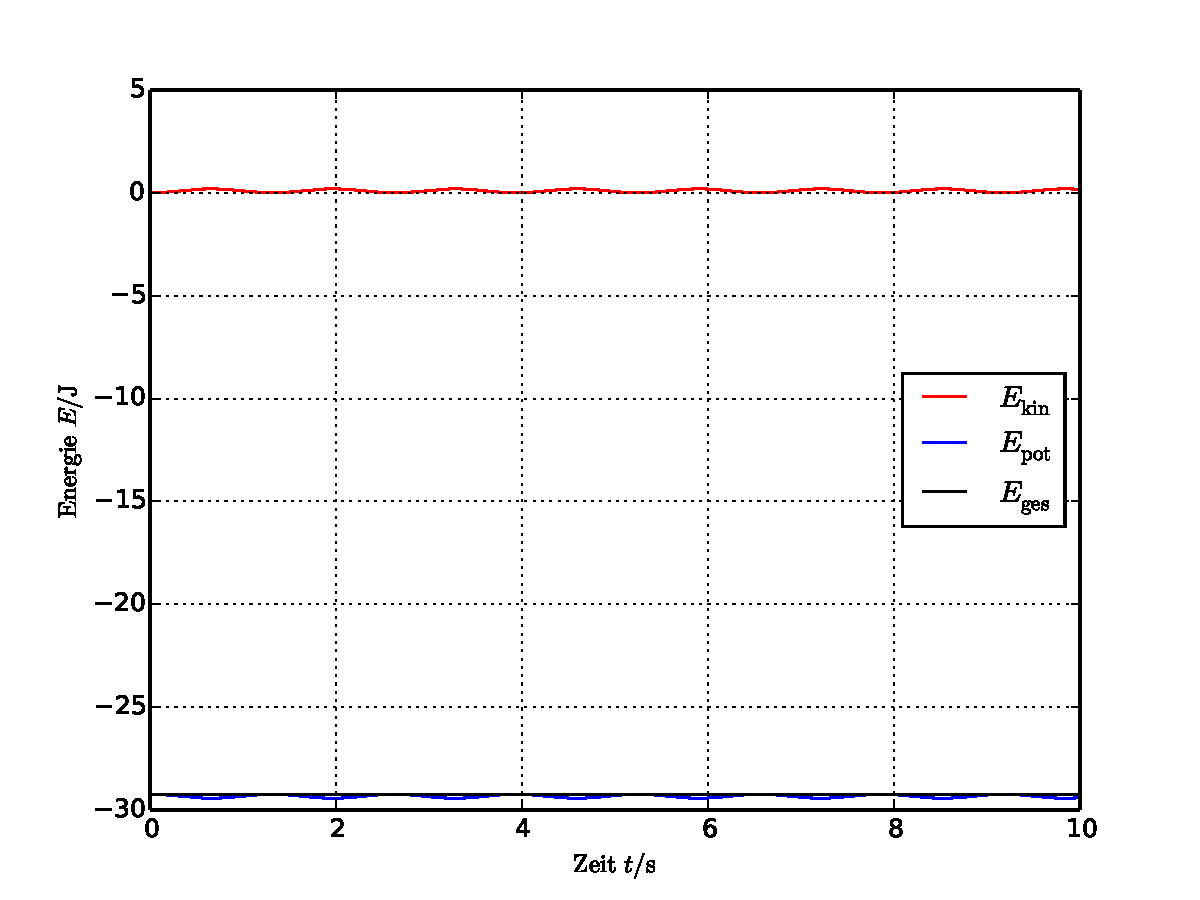
\includegraphics[width = 0.49\textwidth]{../Plots/Plot_1_C_1_energie.pdf}}
	\subfigure[$\theta_2=-\sqrt{2}\theta_1$]{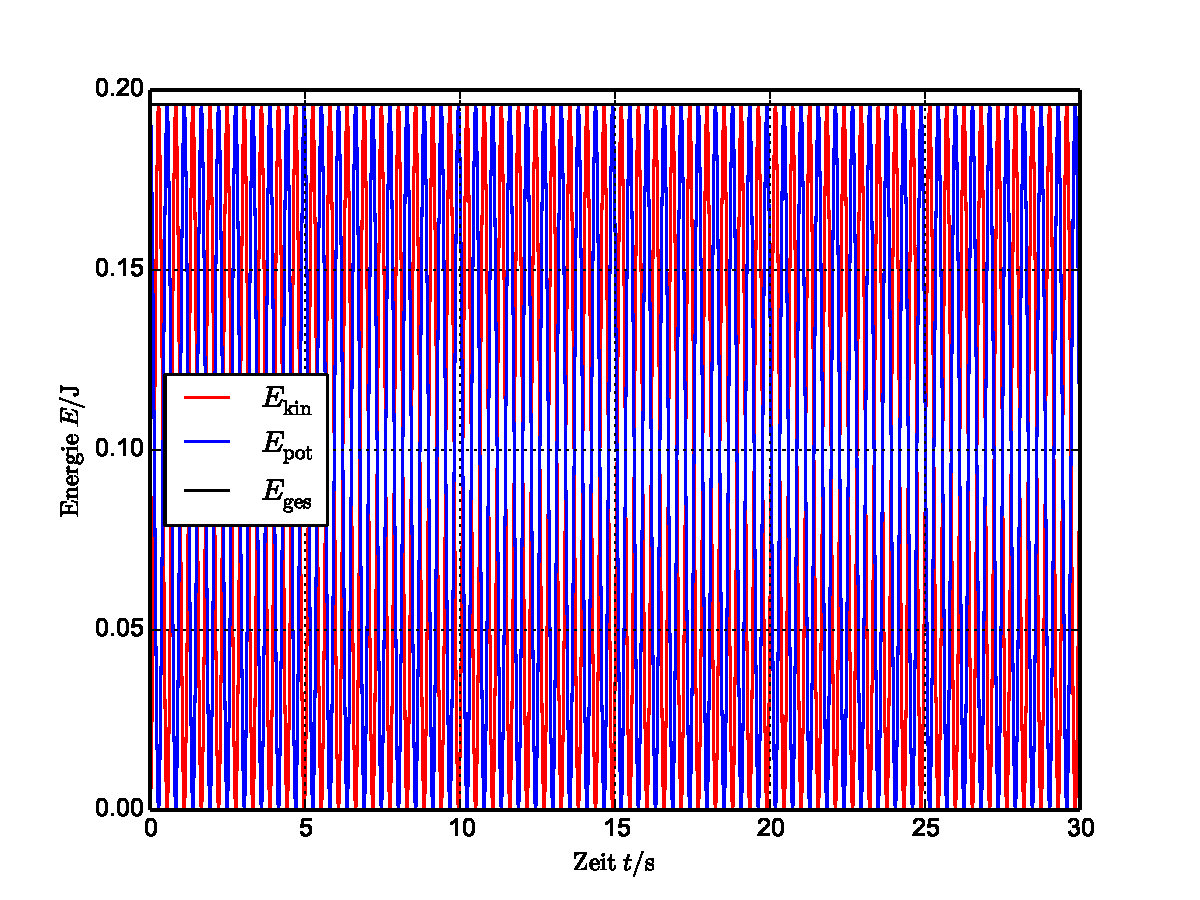
\includegraphics[width = 0.49\textwidth]{../Plots/Plot_1_C_2_energie.pdf}}
	\caption{Kinetische Energie $E_\text{kin}$, potentielle Energie $E_\text{pot}$ und Gesamtenergie $E_\text{ges}$ in Abhängigkeit von der Zeit $t$ mit den unterschiedlichen Anfangsbedingungen.\label{fig:Energie}}
\end{figure}\\
Im Fall von $\theta_2=+\sqrt{2}\theta_1$ geschehen die Schwingungen immer in gleicher Richtung, wohingegen sie im Fall von $\theta_2=-\sqrt{2}\theta_1$ gegenläufig sind.
\begin{figure}[h!]
	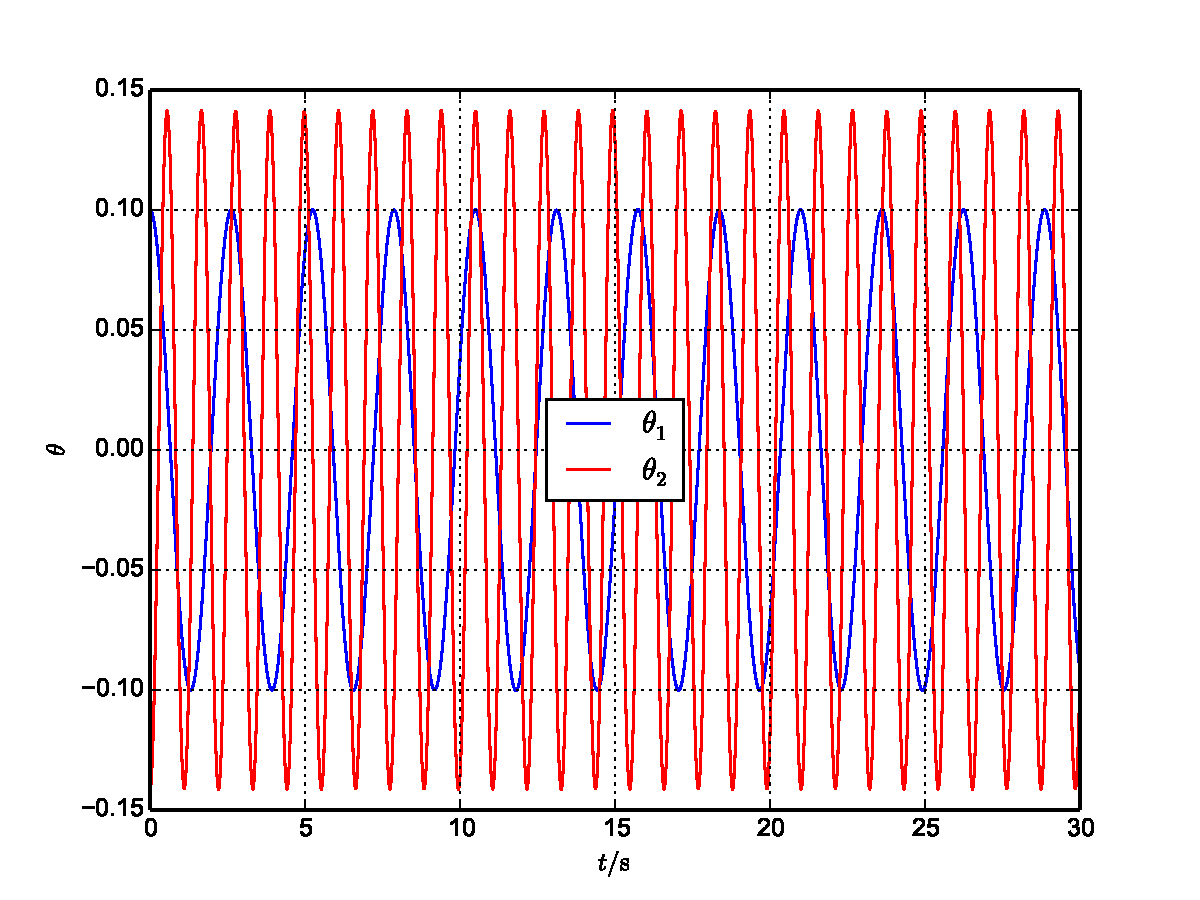
\includegraphics[width = \textwidth]{../Plots/Plot_1_C_winkel.pdf}
	\caption{Zeitlicher Verlauf der Winkel.\label{fig:winkel}}
\end{figure}

\begin{figure}[h!]
	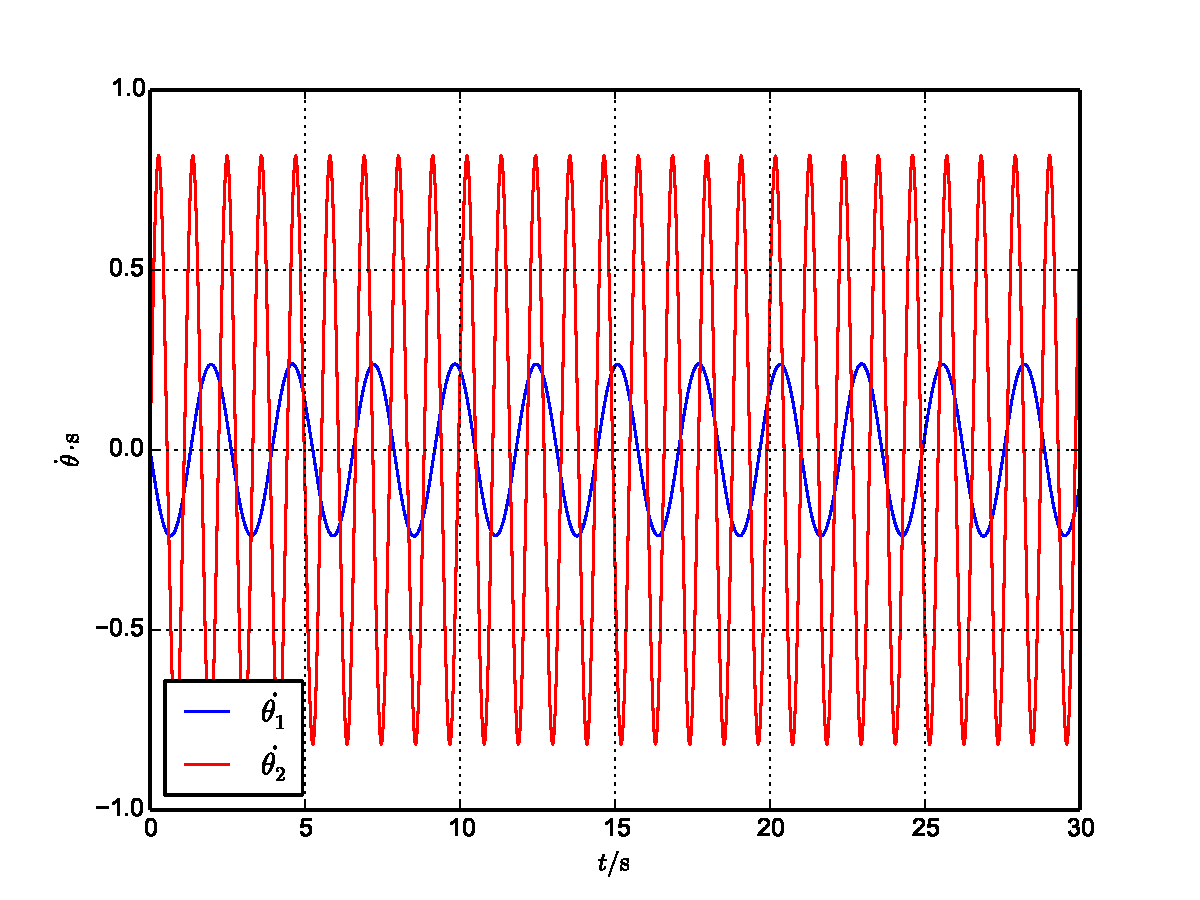
\includegraphics[width = \textwidth]{../Plots/Plot_1_C_winkelgeschwindigkeit.pdf}
	\caption{Zeitlicher Verlauf der Winkelgeschwindigkeit.\label{fig:winkelgeschwindigkeit}}
\end{figure}

\subsection*{d)}
Die Trajektorie der Masse $m_2$ ist in \cref{fig:Trajektorie} dargestellt.
Aufgetragen sind $x$- und $y$-Koordinate des Vektors $\vec{r_2}$ aus Aufgabenteil a).
\begin{figure}[h!]
	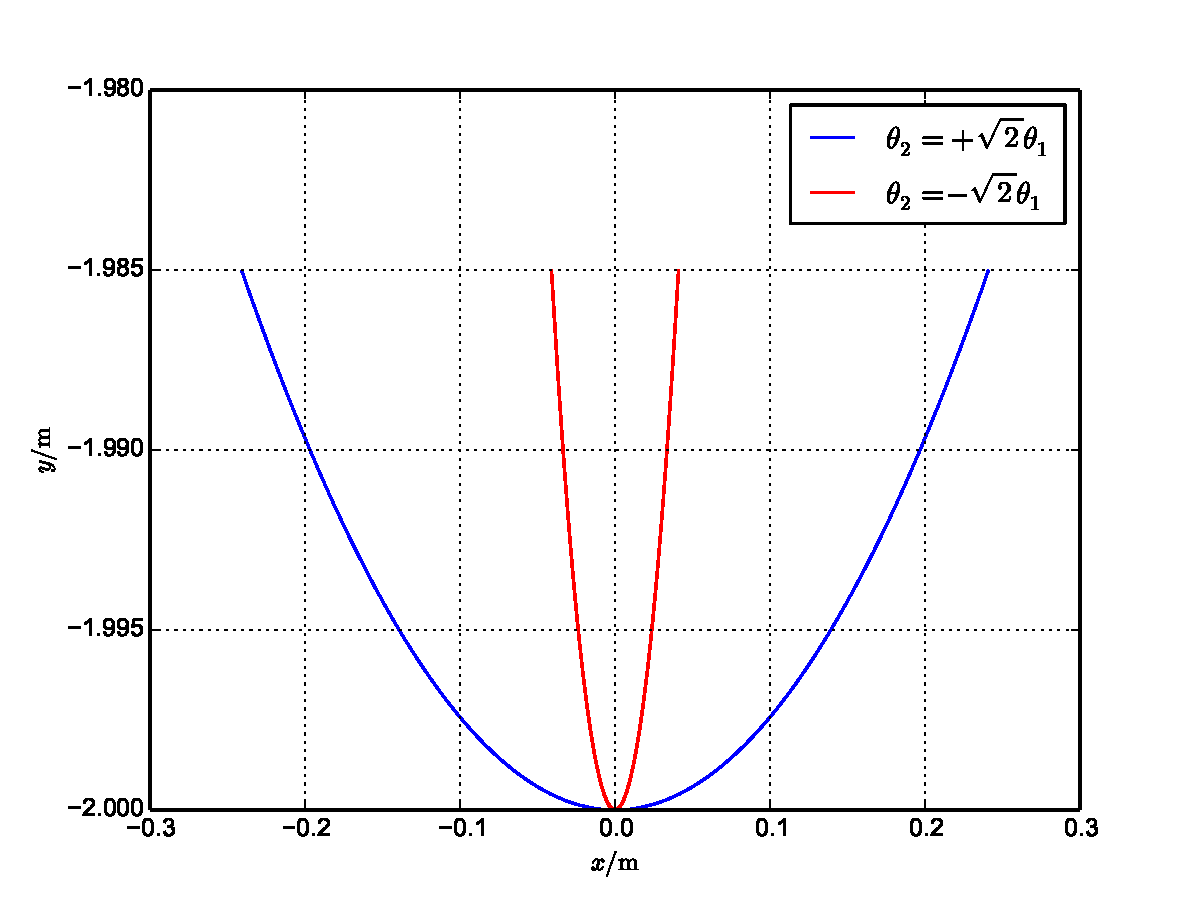
\includegraphics[width = \textwidth]{../Plots/Plot_1_D_trajektorie.pdf}
	\caption{Trajektorie der Masse $m_2$.\label{fig:Trajektorie}}
\end{figure}
